\begin{figure}
\centering

\begin{tabular}{cc}

\begin{subfigure}[b]{0.5\textwidth}
\centering
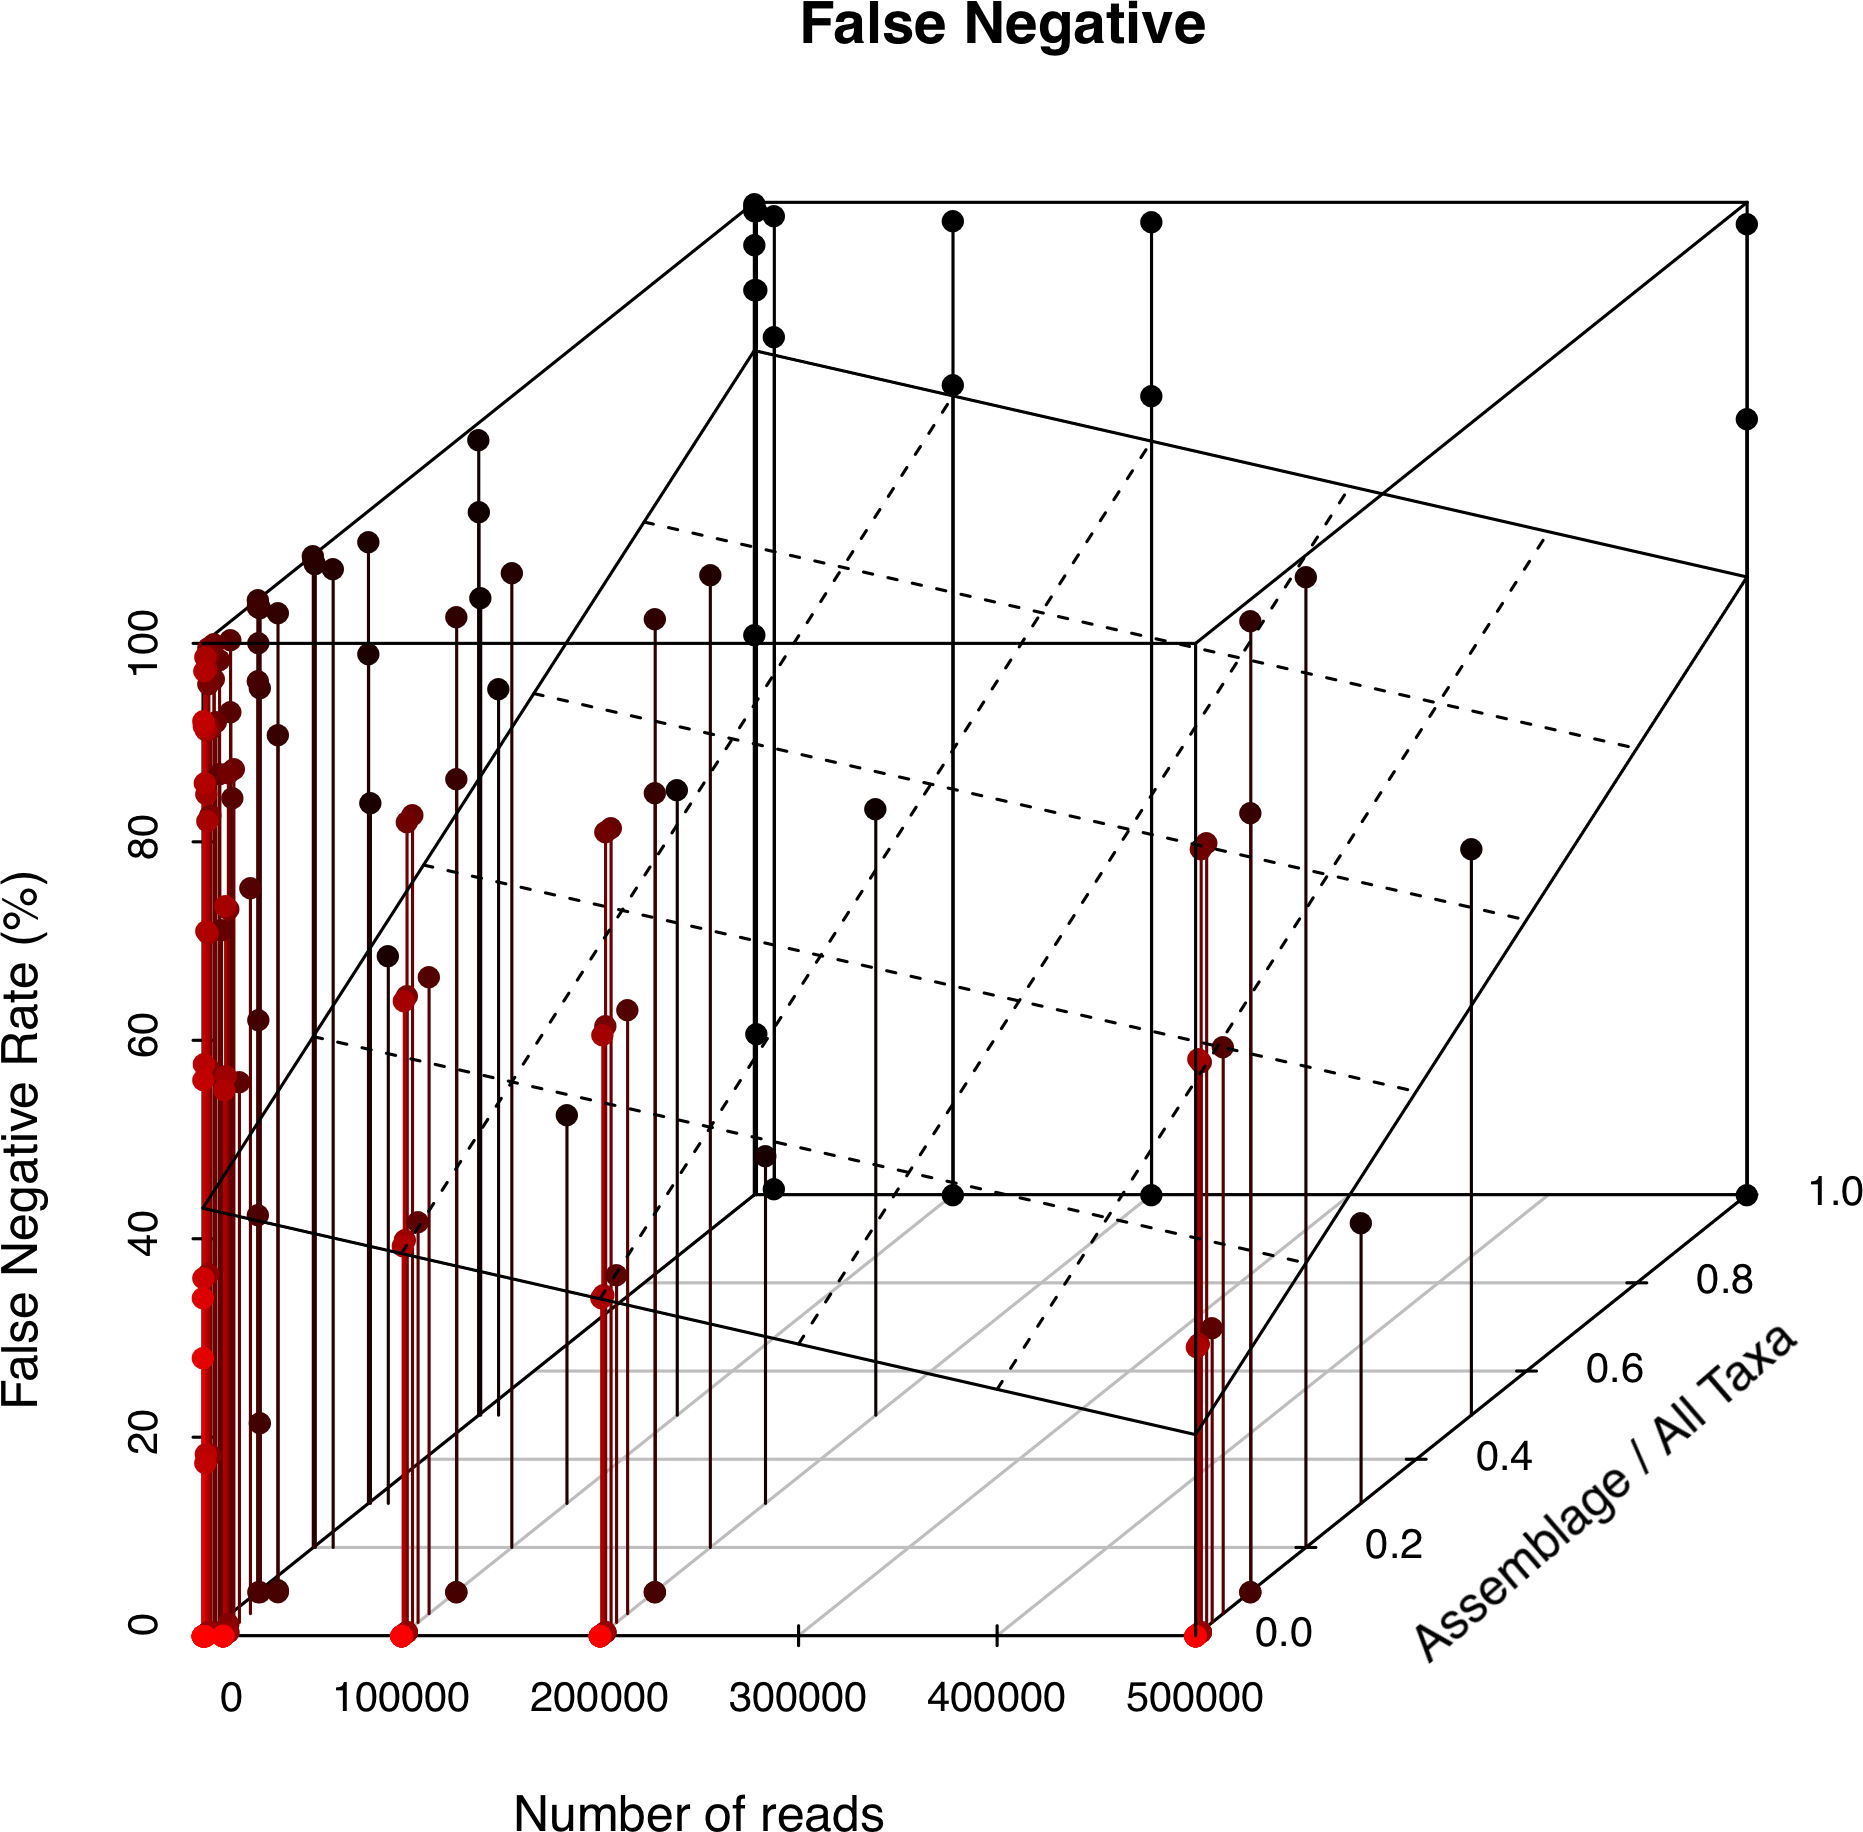
\includegraphics[width=\textwidth]{../polarfront/falsenegative.png}
\caption{TODO false negative}
\label{fig:minspecvalidationfalsenegative}
\end{subfigure}%

&
%\quad %add desired spacing between images, e. g. ~, \quad, \qquad etc. 
%(or a blank line to force the subfigure onto a new line)

\begin{subfigure}[b]{0.5\textwidth}
\centering
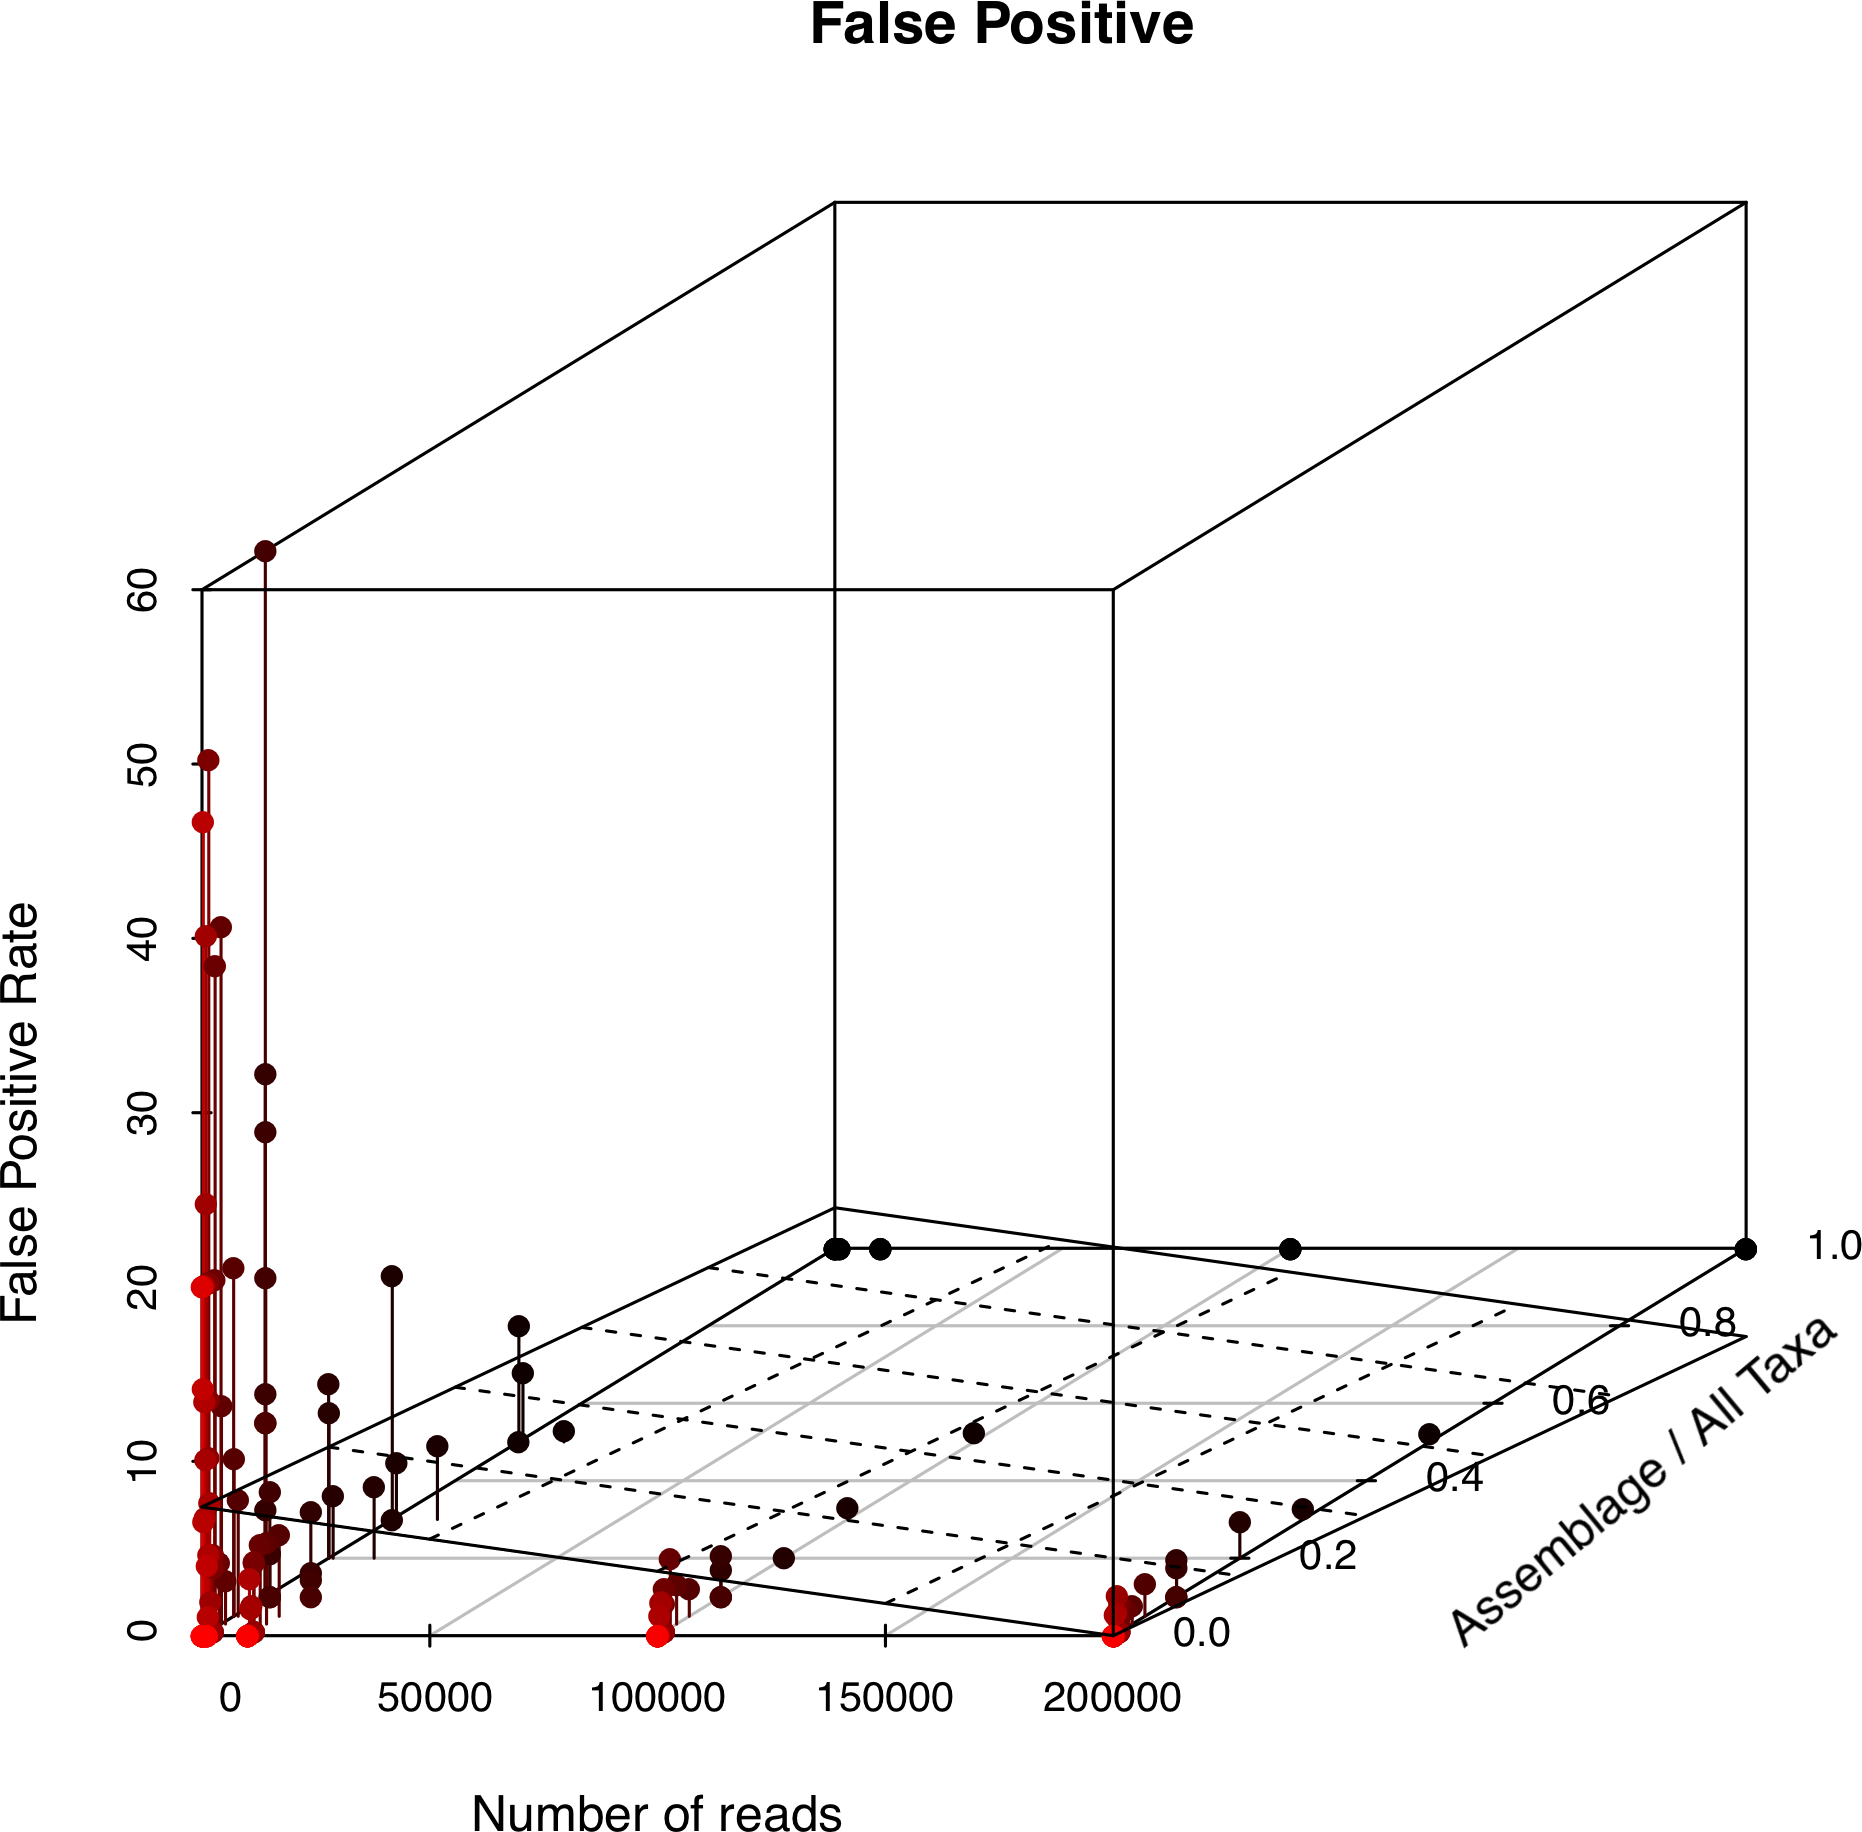
\includegraphics[width=\textwidth]{../polarfront/falsepositive.png}
\caption{TODO false positive}
\label{fig:minspecvalidationfalsepositive}
\end{subfigure}

\\
\bigskip
\\
\bigskip
\\
\bigskip
\\
%\quad %add desired spacing between images, e. g. ~, \quad, \qquad etc. 
%(or a blank line to force the subfigure onto a new line)

\begin{subfigure}[b]{0.5\textwidth}
\centering
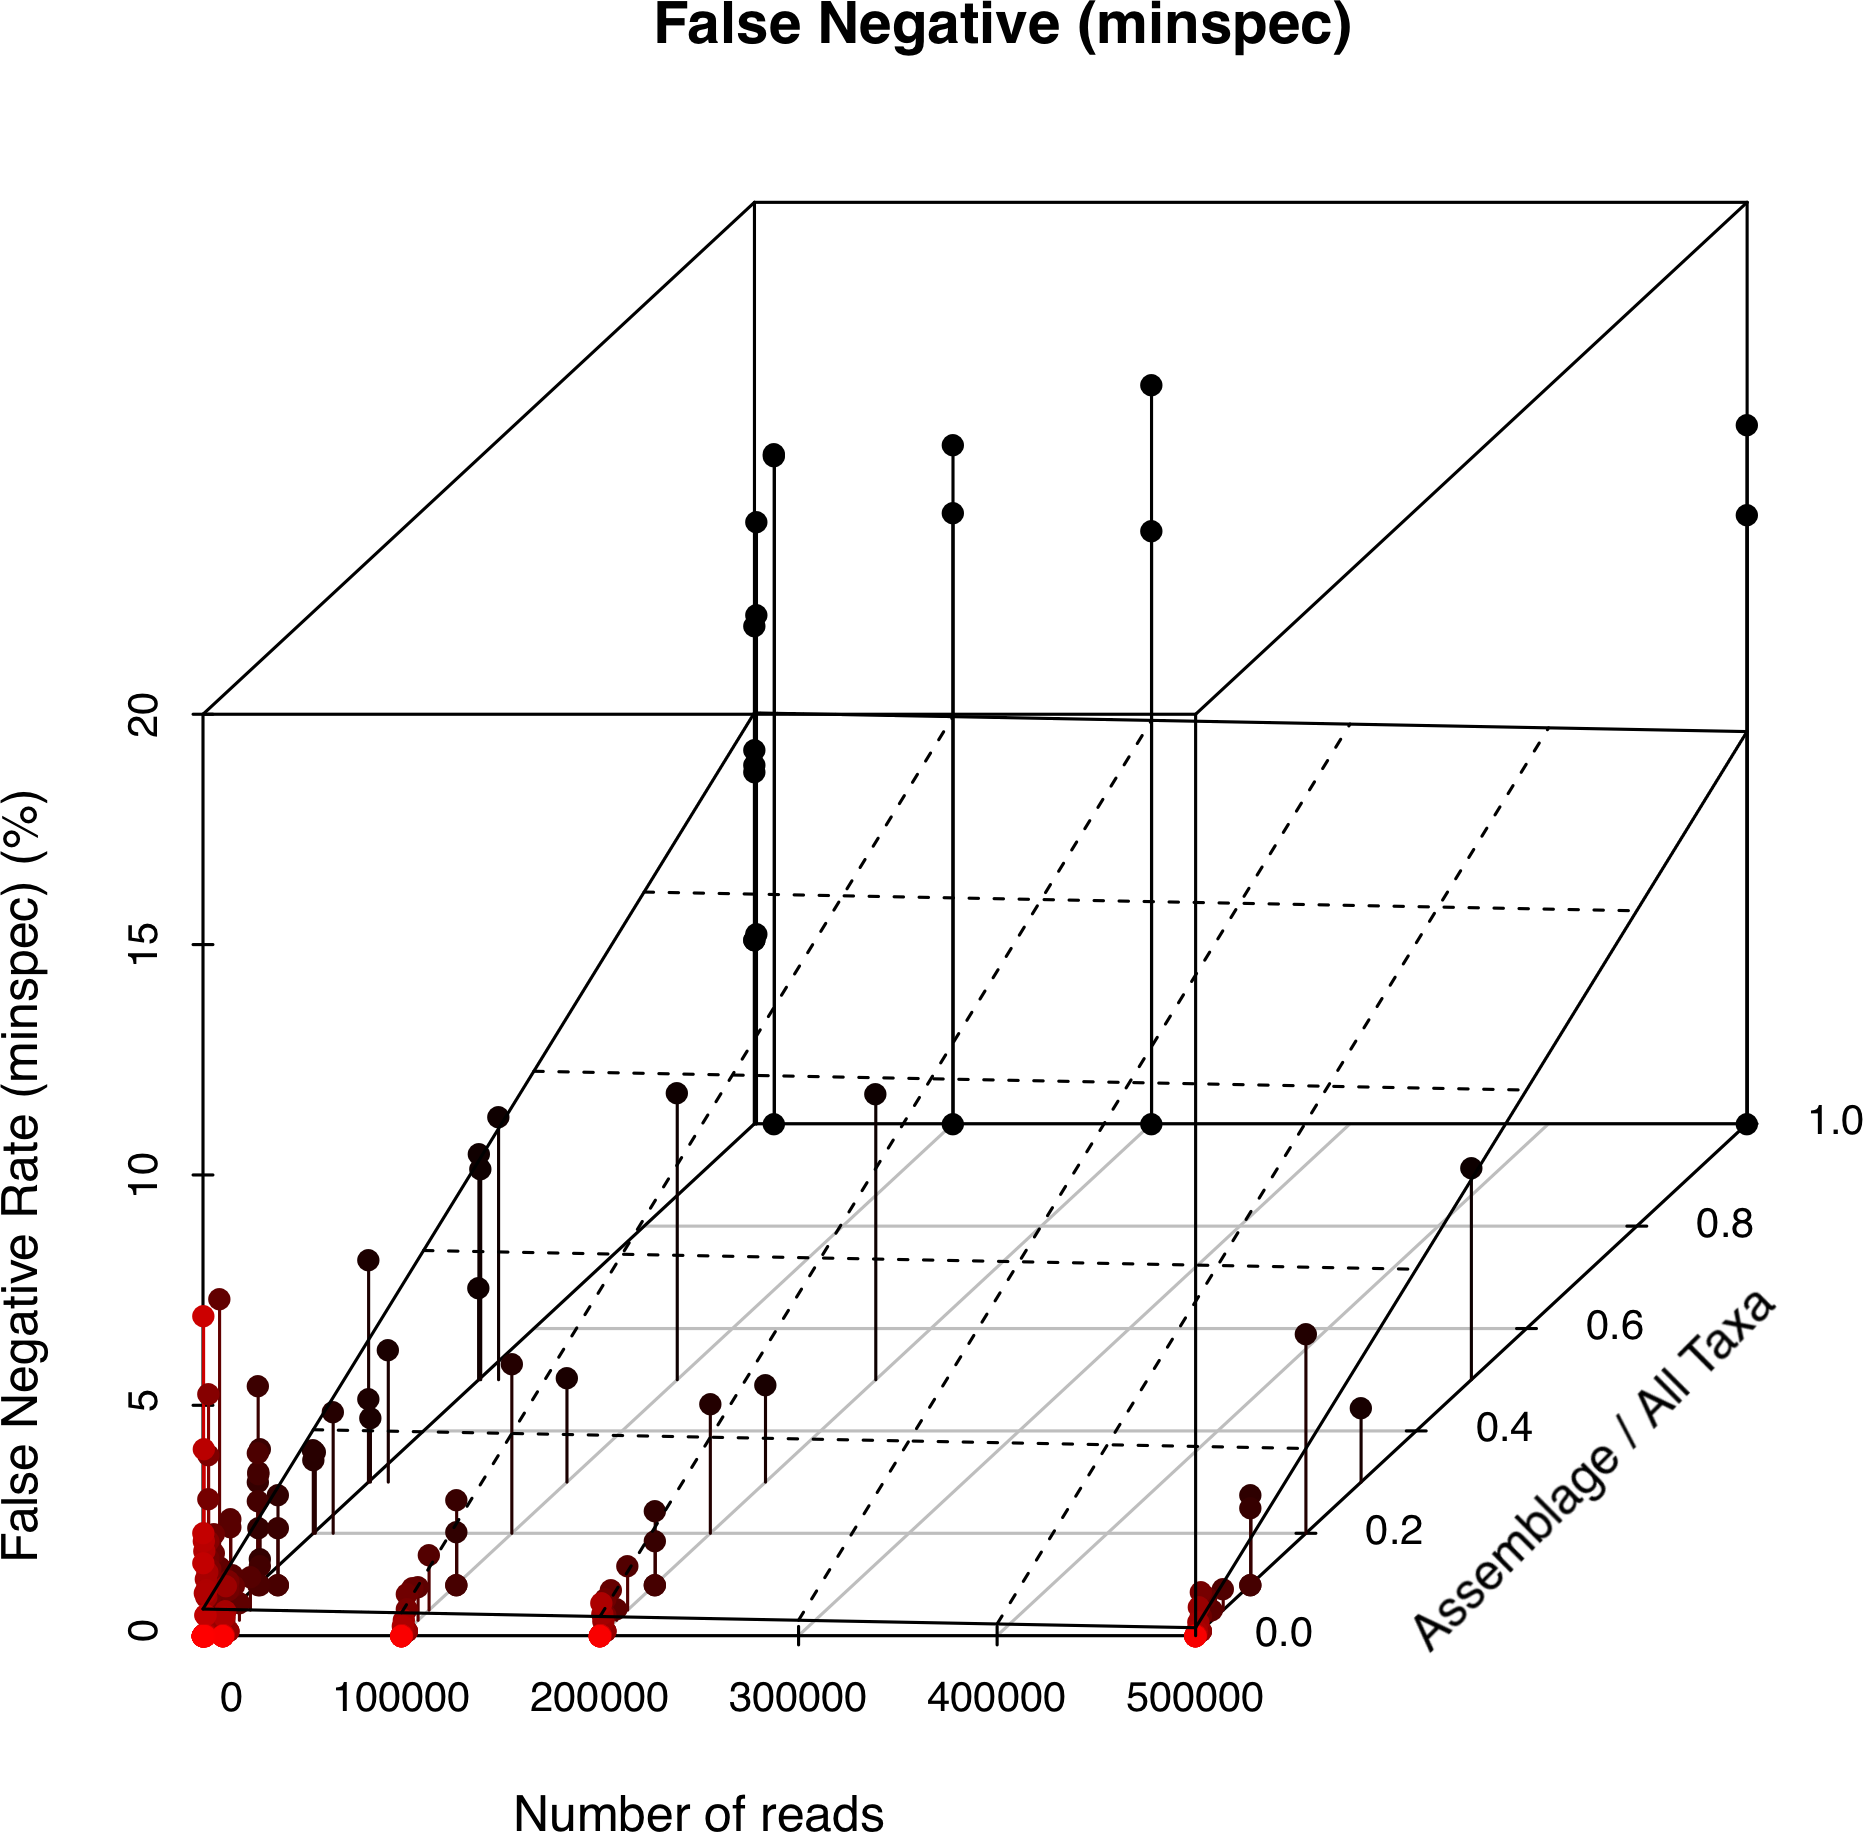
\includegraphics[width=\textwidth]{../polarfront/minspecfalsenegative.png}
\caption{TODO minspec false negative}
\label{fig:minspecvalidationminspecfalsenegative}
\end{subfigure}

&
%\quad %add desired spacing between images, e. g. ~, \quad, \qquad etc. 
%(or a blank line to force the subfigure onto a new line)

\begin{subfigure}[b]{0.5\textwidth}
\centering
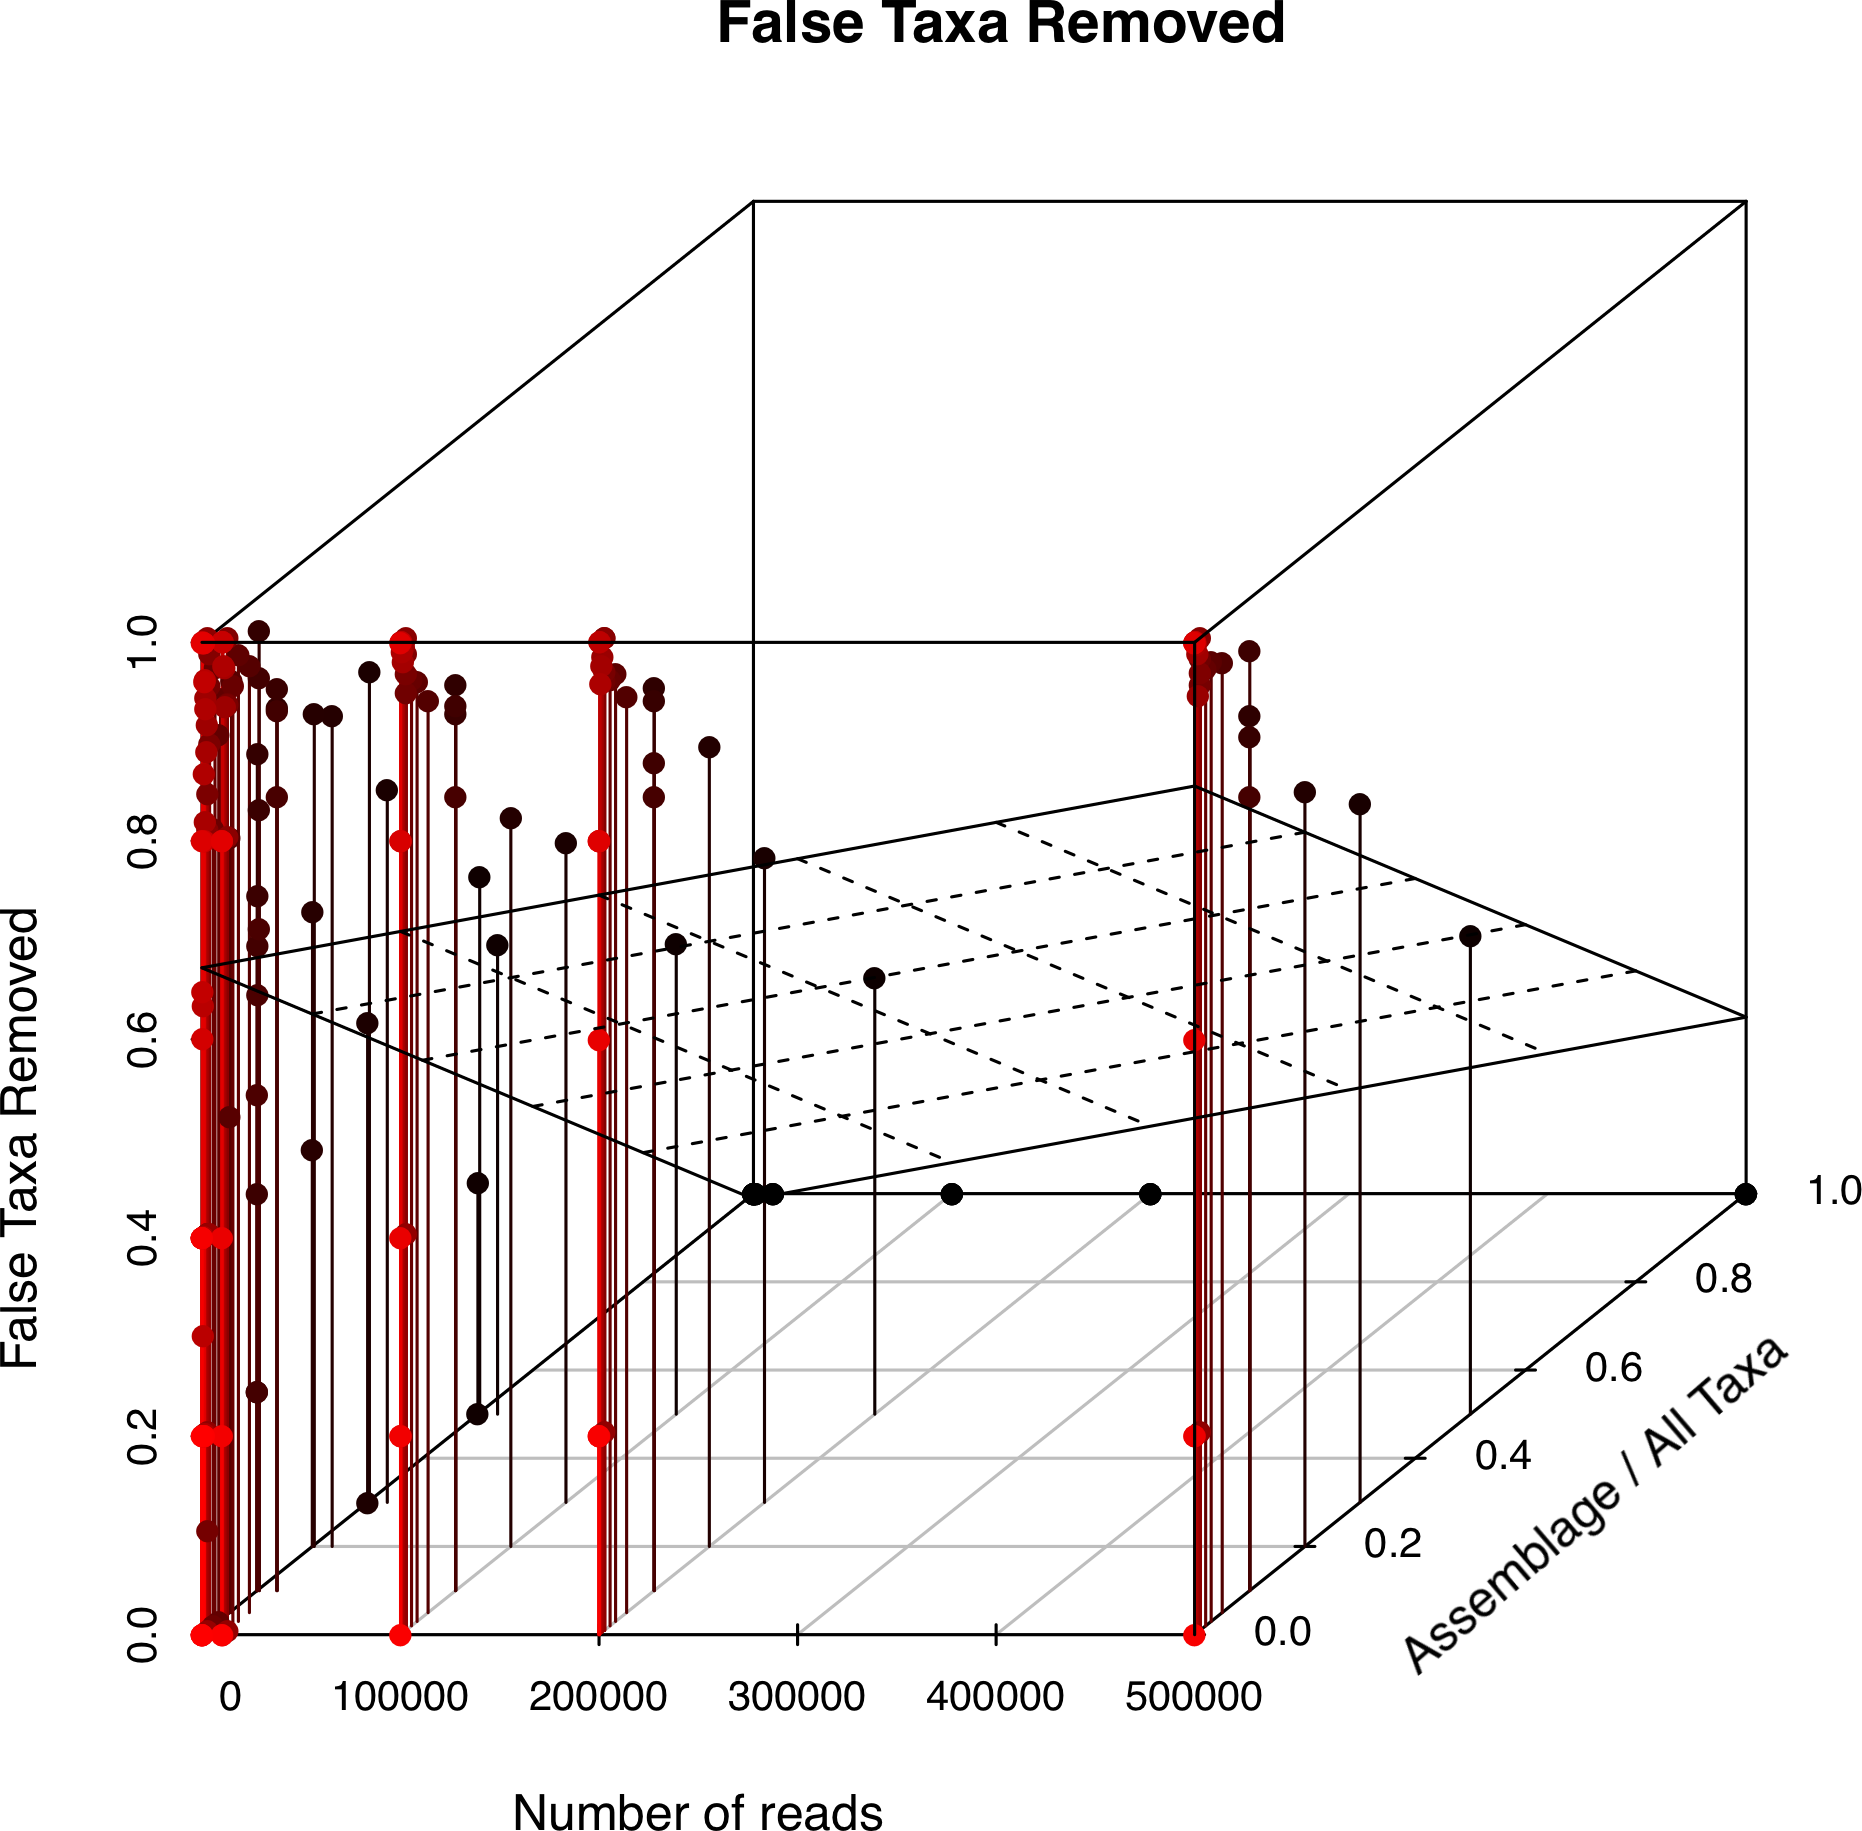
\includegraphics[width=\textwidth]{../polarfront/falsetaxaremoved.png}
\caption{TODO minspec false taxa removed}
\label{fig:minspecvalidationfalsetaxaremoved}
\end{subfigure}
\\

\end{tabular}

\caption{TODO master caption}\label{fig:minspecvalidation}
\end{figure}
